\section{Más}

\begin{frame}[fragile]{Hoogle}
  Hoogle permite buscar funciones por tipo entre las librerías
  estándar de Haskell:

  \begin{center}
  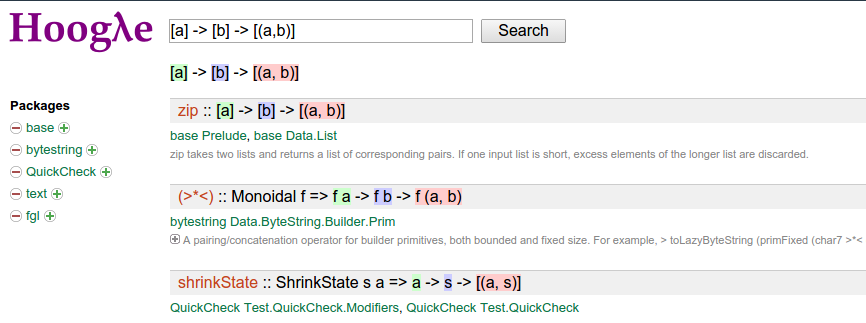
\includegraphics[scale=0.35]{./images/hoogle.png}
  \end{center}
\end{frame}


\begin{frame}[fragile]{Demostraciones}
  Como las funciones no tienen efectos secundarios, podemos razonar la
  corrección del código por inducción:

  \begin{lstlisting}[language=haskell]
qsort []     = []
qsort (x:xs) = qsort [y | y<-xs, y<=x]
            ++ [x]
            ++ qsort [y | y<-xs, y>x]
  \end{lstlisting}

  \textbf{Demostración:} \textit{Quicksort} funciona porque:
  \begin{itemize}
   \item ordena correctamente una lista vacía.
   \item la lista creada mantiene el orden entre las tres partes
  \end{itemize}
\end{frame}


\begin{frame}[fragile]{Idris}
  \textbf{Idris}, construido con Haskell, es un lenguaje
  con su misma sintaxis pero incluyendo tipos dependientes
  para demostrar matemáticamente que los programas son correctos.

  \begin{center}
  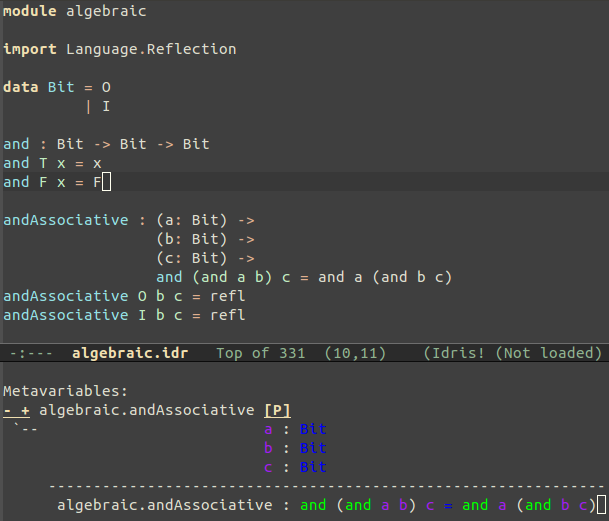
\includegraphics[scale=0.28]{./images/idris.png}
  \end{center}
\end{frame}


\begin{frame}[fragile]{Curry-Howard}
 Los siguientes tipos están habitados:
 \begin{lstlisting}[language=haskell]
 a -> a
 (a,b) -> a
 a -> Either a b
 \end{lstlisting}
 Por las funciones \texttt{id}, \texttt{fst} y \texttt{Left}.
 Estos, sin embargo, no:
 \begin{lstlisting}[language=haskell]
 a -> b
 a -> (a,b)
 Either a b -> a -> b
 \end{lstlisting}

 \textbf{¿Qué tipos de Haskell están habitados?}
 
 \note{No vale que estén habitados para un tipo concreto,
 necesitamos que haya algún elemento general para todos
 los tipos. Es lo que se nota en Haskell como:
 \begin{center}
  \texttt{forall a . a -> a}
 \end{center}
 Necesitamos un elemento de este tipo en lugar de uno como:
 \begin{center}
  \texttt{Int -> Bool}
 \end{center}

 }
\end{frame}


\begin{frame}[fragile]{Curry-Howard}
 A cada tipo le corresponde una proposición lógica, cambiando:
 \begin{itemize}
  \item \texttt{a -> b} por $a \Rightarrow b$
  \item \texttt{(a,b)} por $a \wedge b$
  \item \texttt{Either a b} por $a \vee b$
  \item \texttt{()} por $True$
  \item \texttt{Void} por $False$
 \end{itemize}

 \espacio
 \textbf{¿Qué tipos de Haskell están habitados?} Aquellos cuya
 proposición lógica asociada puede demostrarse verdadera en lógica
 intuicionista.
 
 \note{La lógica intuicionista se creó para el programa constructivista
 de Brouwer. En ella, no se tiene el principio del tercio excluso ni la
 eliminación de la doble negación.}
\end{frame}

\begin{frame}[fragile]{Mónadas}
Las mónadas son constructores de tipos que definen un \textbf{contexto computacional}.
Se definen con:

\espacio

\begin{lstlisting}
return :: a -> m a
\end{lstlisting}
\texttt{return} introduce un valor de tipo \texttt{a} en el contexto.

\espacio

\begin{lstlisting}
>>= :: m a -> (a -> m b) -> m b
\end{lstlisting}
Dado un valor en un contexto y una función que devuelve valores en el contexto,
\textbf{¿Cómo podemos aplicar la función al valor?}-
\end{frame}

\begin{frame}[fragile]{Mónadas: Maybe}
La mónada \texttt{Maybe}, nos permite operar con funciones que pueden \textit{fallar}:

\begin{lstlisting}
return x = Just x -- return = Just
\end{lstlisting}

\espacio

\begin{lstlisting}
Just x  >>= f = f x
Nothing >>= _ = Nothing
\end{lstlisting}
Cuando hay un fallo no devolvemos nada, y cuando no, aplicamos la función al valor
del interior de \texttt{Just}.
\end{frame}

\begin{frame}[fragile]{Mónadas: IO}
\textbf{¿Cómo hacemos E/S con funciones puras?}\\
Utilizamos la mónada \texttt{IO}:

\espacio

\begin{lstlisting}
main = readFile "file1" >>= writeFile "file2"
\end{lstlisting}

\espacio

Todo programa de Haskell se ejecuta evaluando la función \texttt{main}, de tipo
\texttt{IO ()}.

\note{Su implementación es abstracta, pero nos permite componer acciones.}
\end{frame}
